\section{Training the model $f_{\VECTOR{c}}(\VECTOR{x})$}

When we training the model $f_{\VECTOR{c}}(\VECTOR{x})$
our objective is found the vector $\VECTOR{c}=\VECTOR{\hat{c}}$, with the parameters of model, 
that minimise the error when we try fit the model with the training information.
This information is located in 
\begin{itemize}
\item $\MATRIX{I}_c$: The colour image shown in Fig. \ref{fig:data-color}.
\item $\MATRIX{I}_{bw}$: The black and white image shown in Fig. \ref{fig:data-trainning-bw}.
\end{itemize}
The Fig \ref{fig:training} represents this procedure.

\begin{figure}[h!]
\centering
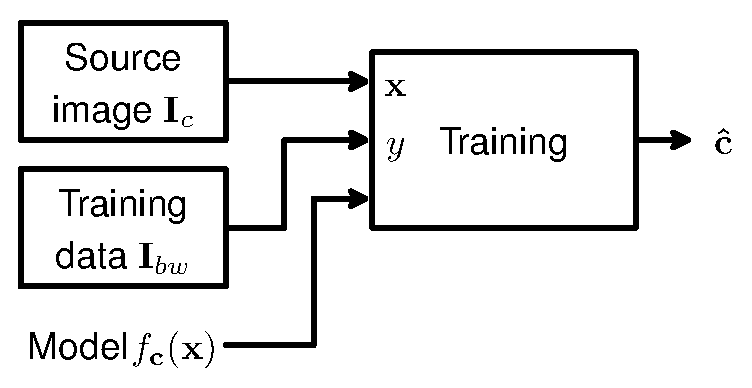
\includegraphics[width=0.99\linewidth]{training.eps}
\caption{Block diagram of model training.}
\label{fig:training}
\end{figure} 

The training block follow the procedure described in the 
Algorithm \ref{alg:alg1}, that additionally need some variables like $\epsilon=0.00005$, $N=11023$ and $K=10$ to work.
\begin{itemize}
\item $\epsilon$: The value $y$ to each pixel $\VECTOR{x}$ chosen in image $\MATRIX{I}_{c}$
with a ``black'' pixel in image $\MATRIX{I}_{bw}$, where $0 < \epsilon \ll 0.5$.
\item $N$: The number of randomly selected points (pixels) 
in each training repetition.
\item $K$: The number of training repetitions.
\end{itemize}

\begin{algorithm}
 \KwData{
$\MATRIX{I}_c$,
$\MATRIX{I}_{bw}$,
$\epsilon$,
$N$,
$K$.
}
 \KwResult{The optimised $\VECTOR{\hat{c}}$ parameter to form the classifier $f_{\VECTOR{\hat{c}}}(\VECTOR{x})$.}~\\
 $\VECTOR{y}=[\underbrace{\epsilon   \quad \hdots \quad \epsilon }_{N~elements} \quad 
\underbrace{ 1-\epsilon \quad \hdots \quad 1-\epsilon }_{N~elements}]^{\transpose}$\;
 \For{$k=1$ \KwTo $K$}{
  $\MATRIX{P}_b=get\_points(\MATRIX{I}_c,\MATRIX{I}_{bw},N,``\mathbf{black}")$\;
  $\MATRIX{P}_w=get\_points(\MATRIX{I}_c,\MATRIX{I}_{bw},N,``\mathbf{white}")$\;
  $\MATRIX{P}=\begin{bmatrix}\MATRIX{P}_b\\ \MATRIX{P}_w \end{bmatrix}$\;
  $\left[\VECTOR{\hat{c}}_k,~e(\VECTOR{\hat{c}}_k)\right]=get\_parameters\left( \MATRIX{P}, \VECTOR{y}\right)$\;
 }
 $\VECTOR{\hat{c}}=\frac{\sum\limits_{k=1}^{K} \frac{\VECTOR{\hat{c}}_k}{e(\VECTOR{\hat{c}}_k)}}{\sum\limits_{k=1}^{K} \frac{1}{e(\VECTOR{\hat{c}}_k)}}$\;
 \caption{Method to get the vector $\VECTOR{\hat{c}}$.}
\label{alg:alg1}
\end{algorithm}

\subsection{Function $get\_points(\MATRIX{I}_c,\MATRIX{I}_{bw},N,TYPE)$}
The function choose randomly\footnote{Follow an uniform distribution.}
$N$ points (pixels) $\VECTOR{x}_n$, $1 \leq n \leq N$,
from the colour image $\MATRIX{I}_c$,
with the condition that each point selected in $\MATRIX{I}_c$ need be of type $TYPE$
in the same position of image $\MATRIX{I}_{bw}$;
where $TYPE \in \{``\mathbf{black}",``\mathbf{white}"\}$. 
Thus, the function return the matrix $\MATRIX{P} \in \mathbb{R}^{N \times 3}$,
\begin{equation}
\MATRIX{P}=
\begin{bmatrix}
\VECTOR{x}_1^{\transpose}  \\
%\VECTOR{x}_2^{\transpose}  \\
\vdots  \\
\VECTOR{x}_n^{\transpose}  \\
\vdots \\
\VECTOR{x}_N^{\transpose} \\
\end{bmatrix},
\end{equation} 
with the information of $N$ randomly selected black or white points.

\subsection{Function $get\_parameters\left( \MATRIX{P}, \VECTOR{y}\right)$}
Given, a group of $L$ points
$\VECTOR{x}_l \in \mathbb{R}^{3}$,
labelled with the values $y_l \in \mathbb{R}$, $1\leq l \leq L$;
ordering in the matrices $\MATRIX{P} \in \mathbb{R}^{L \times 3}$ and 
$\VECTOR{Y} \in \mathbb{R}^{L}$ respectively,
\begin{equation}
\MATRIX{P}=
\begin{bmatrix}
\VECTOR{x}_1^{\transpose}  \\
%\VECTOR{x}_2^{\transpose}  \\
\vdots  \\
\VECTOR{x}_l^{\transpose}  \\
\vdots \\
\VECTOR{x}_L^{\transpose} \\
\end{bmatrix},
\quad 
\VECTOR{y}=
\begin{bmatrix}
y_1  \\
%y_2  \\
\vdots  \\
y_l  \\
\vdots \\
y_L \\
\end{bmatrix};
\end{equation}
if we want to create a classifier using the function $f_{\VECTOR{c}}(\VECTOR{x})$,
with domain $\VECTOR{x} \in \mathbb{R}^{3}$, range $y \in \mathbb{R}$ and
parameters grouped in the vector $\VECTOR{c}\in \mathbb{R}^{4}$,
as defined in Eq. (\ref{eq:reglogrnr1:1}),
\begin{equation}\label{eq:reglogrnr1:1}
y=f_{\VECTOR{c}}(\VECTOR{x}),
\end{equation}
or your equivalent
\begin{equation}\label{eq:logitfunc}
logit(y)=h_{\VECTOR{c}}(\VECTOR{x}),
\end{equation}
where $logit(y) \equiv ln\left( \frac{y}{1-y}\right)$.
We can affirm that 
the vector $\VECTOR{c}= \VECTOR{\hat{c}}$
that fit the model $f_{\VECTOR{c}}$ between the samples $\VECTOR{x}_l$ and the labels $y_l$,
and minimise the square error $e(\VECTOR{c})$,
\begin{equation}\label{eq:reglogrnr1:1e}
\begin{array}{lll}
e(\VECTOR{c}) & = & \frac{1}{L}\sum\limits_{l=1}^{L} ||h_{\VECTOR{c}}(\VECTOR{x}_l)-logit(y_l)||^2,\\
            ~ & = & \frac{1}{L}\sum\limits_{l=1}^{L} ||\left[1\quad \VECTOR{x}_l^{\transpose}\right]\VECTOR{c}-logit(y_l)||^2,\\
            ~ & = & \frac{1}{L}||\MATRIX{A}\VECTOR{c}-\VECTOR{z}||^2,
\end{array}
\end{equation}
\begin{equation}
\MATRIX{A}=
\begin{bmatrix}
1 & \VECTOR{x}_1^{\transpose}\\
%1 & \VECTOR{x}_2^{\transpose}\\
\vdots & \vdots\\
1 & \VECTOR{x}_l^{\transpose}\\
\vdots & \vdots\\
1 & \VECTOR{x}_L^{\transpose}\\ 
\end{bmatrix},
\quad
\VECTOR{z}=
\begin{bmatrix}
logit(y_1)  \\
%logit(y_2)  \\
\vdots  \\
logit(y_l)  \\
\vdots \\
logit(y_L) \\
\end{bmatrix},
\end{equation}
can be found by the Eq. (\ref{eq:reglogrnr1:2}), 
\begin{equation}\label{eq:reglogrnr1:2}
\VECTOR{\hat{c}} = \left[ \MATRIX{A}^{\transpose} \MATRIX{A}\right]^{-1} \MATRIX{A}^{\transpose} \VECTOR{z},\\
\end{equation}
and affirm that $[\VECTOR{\hat{c}},~e(\VECTOR{\hat{c}})]=get\_parameters\left( \MATRIX{P}, \VECTOR{y}\right)$.

